This section reports estimates of treatment effects for the main outcomes by gender, tests of equality of effects by outcome, and the estimated combining functions. These estimates show that the program treatment effects are strong for both males and females are that treatment effects depend on the counterfactual against which they are benchmarked (home or low quality center care). Treatment effects sharply differ by gender.

\subsection{Estimated Treatment Effects}

Tables~\ref{table:tescombinedmales} and \ref{table:tescombinedfemales} present the estimates of a representative selection of the main treatment effects for males and females respectively. The full list of treatment effects is reported in Web Appendix~\ref{appendix:results}. Column (1) of each table gives sample mean differences in outcomes between treatment and control groups. Column (2) adjusts the differences for attrition and controls for background variables. Both are estimates of the parameter defined in equation~\eqref{eq:effect}, but with different conditioning sets. Column (3) shows the mean difference between the full treatment-group and the control-group subjects who did not attend alternative preschools. Column (4) gives standard matching estimates for the parameter defined in equation~\eqref{eq:influenza}.\footnote{In Appendix~\ref{app:matching-is-fun}, we provide details on: (i) the kernel matching estimator that we use; (ii) the matching variables that we use; and (iii) a sensitivity analysis to these matching variables.} Column (5) reports estimates of the parameter defined by equation~\eqref{eq:smallpox}. mean differences between the full treatment-group and control-group children who attended alternatives. Column (6) gives matching estimates for the parameter of equation~\eqref{eq:smallpox}.

The results for females show that ABC/CARE has substantial effects on education when comparing outcomes of the treatment-group subjects to those from the next best alternative. High school graduation increases between 13 and 25 percentage points, depending on the estimate that we consider; college graduation increases 13 percentage points; and the average years of schooling increase between 2.1 and 1.8 years. Employment at age 30 increases between 13 and 8 percentage points. ABC/CARE has substantial impacts on human capital accumulation and employment. The results strengthen when we compare treatment with the option of staying at home.

\begin{sidewaystable}[!htbp]
\centering
\begin{threeparttable}
\caption{Treatment Effects on Selected Outcomes, Males}\label{table:tescombinedmales}
\begin{scriptsize}
  \begin{tabular}{cccccccccccc}
  \toprule
   Category & Variable & Age & $\bar{Y}_C$ & (1) & (2) & (3) & (4) & (5) & (6) \\

    \midrule
    % cat 3
     \mc{1}{l}{\scriptsize{Parental Income}} &   \mc{1}{l}{\scriptsize{Parental Labor Income}} & \mc{1}{c}{\scriptsize{3.5}} & \mc{1}{c}{\scriptsize{13,505}} & \mc{1}{c}{\scriptsize{1,036}} & \mc{1}{c}{\scriptsize{494}} & \mc{1}{c}{\scriptsize{73.862}} & \mc{1}{c}{\scriptsize{1,462}} & \mc{1}{c}{\scriptsize{123}} & \mc{1}{c}{\scriptsize{690}} \\  

  &   &  & & \mc{1}{c}{\scriptsize{(0.374)}} & \mc{1}{c}{\scriptsize{(0.411)}} & \mc{1}{c}{\scriptsize{(0.474)}} & \mc{1}{c}{\scriptsize{(0.390)}} & \mc{1}{c}{\scriptsize{(0.479)}} & \mc{1}{c}{\scriptsize{(0.417)}} \\  

  &   & \mc{1}{c}{\scriptsize{12}} & \mc{1}{c}{\scriptsize{23,868}} & \mc{1}{c}{\scriptsize{7,085}} & \mc{1}{c}{\scriptsize{9,625}} & \mc{1}{c}{\scriptsize{18,050}} & \mc{1}{c}{\scriptsize{12,639}} & \mc{1}{c}{\scriptsize{6,620}} & \mc{1}{c}{\scriptsize{5,383}} \\  

  &   &  & & \mc{1}{c}{\scriptsize{\textbf{(0.092)}}} & \mc{1}{c}{\scriptsize{\textbf{(0.020)}}} & \mc{1}{c}{\scriptsize{\textbf{(0.038)}}} & \mc{1}{c}{\scriptsize{\textbf{(0.074)}}} & \mc{1}{c}{\scriptsize{\textbf{(0.098)}}} & \mc{1}{c}{\scriptsize{(0.139)}} \\  

  &   & \mc{1}{c}{\scriptsize{15}} & \mc{1}{c}{\scriptsize{22,985}} & \mc{1}{c}{\scriptsize{8,488}} & \mc{1}{c}{\scriptsize{4,495}} & \mc{1}{c}{\scriptsize{5,540}} & \mc{1}{c}{\scriptsize{4,805}} & \mc{1}{c}{\scriptsize{2,885}} & \mc{1}{c}{\scriptsize{4,345}} \\  

  &   &  & & \mc{1}{c}{\scriptsize{\textbf{(0.071)}}} & \mc{1}{c}{\scriptsize{(0.221)}} & \mc{1}{c}{\scriptsize{(0.243)}} & \mc{1}{c}{\scriptsize{(0.264)}} & \mc{1}{c}{\scriptsize{(0.354)}} & \mc{1}{c}{\scriptsize{(0.296)}} \\  

  &   & \mc{1}{c}{\scriptsize{21}} & \mc{1}{c}{\scriptsize{21,585}} & \mc{1}{c}{\scriptsize{12,732}} & \mc{1}{c}{\scriptsize{8,809}} & \mc{1}{c}{\scriptsize{122}} & \mc{1}{c}{\scriptsize{-933}} & \mc{1}{c}{\scriptsize{10,784}} & \mc{1}{c}{\scriptsize{10,283}} \\  

  &   &  & & \mc{1}{c}{\scriptsize{\textbf{(0.005)}}} & \mc{1}{c}{\scriptsize{\textbf{(0.098)}}} & \mc{1}{c}{\scriptsize{(0.448)}} & \mc{1}{c}{\scriptsize{(0.456)}} & \mc{1}{c}{\scriptsize{\textbf{(0.056)}}} & \mc{1}{c}{\scriptsize{\textbf{(0.041)}}} \\  

   \mc{1}{l}{\scriptsize{Education}} &   \mc{1}{l}{\scriptsize{Graduated High School}} & \mc{1}{c}{\scriptsize{30}} & \mc{1}{c}{\scriptsize{0.600}} & \mc{1}{c}{\scriptsize{0.073}} & \mc{1}{c}{\scriptsize{0.044}} & \mc{1}{c}{\scriptsize{0.116}} & \mc{1}{c}{\scriptsize{0.083}} & \mc{1}{c}{\scriptsize{0.040}} & \mc{1}{c}{\scriptsize{0.063}} \\  

  &   &  & & \mc{1}{c}{\scriptsize{(0.262)}} & \mc{1}{c}{\scriptsize{(0.375)}} & \mc{1}{c}{\scriptsize{\textbf{(0.001)}}} & \mc{1}{c}{\scriptsize{(0.346)}} & \mc{1}{c}{\scriptsize{(0.407)}} & \mc{1}{c}{\scriptsize{(0.317)}} \\  

  &  \mc{1}{l}{\scriptsize{Graduated 4-year College}} & \mc{1}{c}{\scriptsize{30}} & \mc{1}{c}{\scriptsize{0.120}} & \mc{1}{c}{\scriptsize{0.170}} & \mc{1}{c}{\scriptsize{0.138}} & \mc{1}{c}{\scriptsize{0.149}} & \mc{1}{c}{\scriptsize{0.099}} & \mc{1}{c}{\scriptsize{0.135}} & \mc{1}{c}{\scriptsize{0.143}} \\  

  &   &  & & \mc{1}{c}{\scriptsize{\textbf{(0.055)}}} & \mc{1}{c}{\scriptsize{(0.128)}} & \mc{1}{c}{\scriptsize{(0.216)}} & \mc{1}{c}{\scriptsize{(0.338)}} & \mc{1}{c}{\scriptsize{(0.154)}} & \mc{1}{c}{\scriptsize{(0.130)}} \\  

  &  \mc{1}{l}{\scriptsize{Years of Education}} & \mc{1}{c}{\scriptsize{30}} & \mc{1}{c}{\scriptsize{12.867}} & \mc{1}{c}{\scriptsize{0.525}} & \mc{1}{c}{\scriptsize{0.541}} & \mc{1}{c}{\scriptsize{1.010}} & \mc{1}{c}{\scriptsize{0.777}} & \mc{1}{c}{\scriptsize{0.351}} & \mc{1}{c}{\scriptsize{0.344}} \\  

  &   &  & & \mc{1}{c}{\scriptsize{(0.151)}} & \mc{1}{c}{\scriptsize{(0.163)}} & \mc{1}{c}{\scriptsize{(0.998)}} & \mc{1}{c}{\scriptsize{(0.136)}} & \mc{1}{c}{\scriptsize{(0.280)}} & \mc{1}{c}{\scriptsize{(0.256)}} \\  

   \mc{1}{l}{\scriptsize{Labor Income}} &   \mc{1}{l}{\scriptsize{Employed}} & \mc{1}{c}{\scriptsize{30}} & \mc{1}{c}{\scriptsize{0.700}} & \mc{1}{c}{\scriptsize{0.119}} & \mc{1}{c}{\scriptsize{0.196}} & \mc{1}{c}{\scriptsize{0.108}} & \mc{1}{c}{\scriptsize{0.040}} & \mc{1}{c}{\scriptsize{0.237}} & \mc{1}{c}{\scriptsize{0.261}} \\  

 &    &  & & \mc{1}{c}{\scriptsize{(0.128)}} & \mc{1}{c}{\scriptsize{\textbf{(0.025)}}} & \mc{1}{c}{\scriptsize{\textbf{(0.001)}}} & \mc{1}{c}{\scriptsize{(0.383)}} & \mc{1}{c}{\scriptsize{\textbf{(0.025)}}} & \mc{1}{c}{\scriptsize{\textbf{(0.013)}}} \\  

  &  \mc{1}{l}{\scriptsize{Labor Income}} & \mc{1}{c}{\scriptsize{30}} & \mc{1}{c}{\scriptsize{30,079}} & \mc{1}{c}{\scriptsize{19,810}} & \mc{1}{c}{\scriptsize{24,365}} & \mc{1}{c}{\scriptsize{25,220}} & \mc{1}{c}{\scriptsize{20,611}} & \mc{1}{c}{\scriptsize{23,072}} & \mc{1}{c}{\scriptsize{21,836}} \\  

   &  &  & & \mc{1}{c}{\scriptsize{\textbf{(0.091)}}} & \mc{1}{c}{\scriptsize{\textbf{(0.092)}}} & \mc{1}{c}{\scriptsize{(0.998)}} & \mc{1}{c}{\scriptsize{(0.122)}} & \mc{1}{c}{\scriptsize{(0.107)}} & \mc{1}{c}{\scriptsize{\textbf{(0.094)}}} \\  

  \mc{1}{l}{\scriptsize{Crime}} &    \mc{1}{l}{\scriptsize{Total Felony Arrests}} & \mc{1}{c}{\scriptsize{Mid-30s}} & \mc{1}{c}{\scriptsize{1.370}} & \mc{1}{c}{\scriptsize{0.196}} & \mc{1}{c}{\scriptsize{0.685}} & \mc{1}{c}{\scriptsize{1.523}} & \mc{1}{c}{\scriptsize{1.340}} & \mc{1}{c}{\scriptsize{0.481}} & \mc{1}{c}{\scriptsize{0.188}} \\  

   &  &  & & \mc{1}{c}{\scriptsize{(0.368)}} & \mc{1}{c}{\scriptsize{(0.183)}} & \mc{1}{c}{\scriptsize{\textbf{(0.064)}}} & \mc{1}{c}{\scriptsize{\textbf{(0.026)}}} & \mc{1}{c}{\scriptsize{(0.284)}} & \mc{1}{c}{\scriptsize{(0.410)}} \\  

  &  \mc{1}{l}{\scriptsize{Total Misdemeanor Arrests}} & \mc{1}{c}{\scriptsize{Mid-30s}} & \mc{1}{c}{\scriptsize{1.296}} & \mc{1}{c}{\scriptsize{-0.501}} & \mc{1}{c}{\scriptsize{-0.244}} & \mc{1}{c}{\scriptsize{-0.298}} & \mc{1}{c}{\scriptsize{-0.034}} & \mc{1}{c}{\scriptsize{-0.246}} & \mc{1}{c}{\scriptsize{-0.507}} \\  

  &   &  & & \mc{1}{c}{\scriptsize{(0.171)}} & \mc{1}{c}{\scriptsize{(0.289)}} & \mc{1}{c}{\scriptsize{(0.314)}} & \mc{1}{c}{\scriptsize{(0.422)}} & \mc{1}{c}{\scriptsize{(0.329)}} & \mc{1}{c}{\scriptsize{(0.168)}} \\  

   \mc{1}{l}{\scriptsize{Health}} &   \mc{1}{l}{\scriptsize{Self-reported drug user}} & \mc{1}{c}{\scriptsize{Mid-30s}} & \mc{1}{c}{\scriptsize{0.500}} & \mc{1}{c}{\scriptsize{-0.333}} & \mc{1}{c}{\scriptsize{-0.438}} & \mc{1}{c}{\scriptsize{-0.673}} & \mc{1}{c}{\scriptsize{-0.557}} & \mc{1}{c}{\scriptsize{-0.326}} & \mc{1}{c}{\scriptsize{-0.330}} \\  

   &  &  & & \mc{1}{c}{\scriptsize{\textbf{(0.019)}}} & \mc{1}{c}{\scriptsize{\textbf{(0.002)}}} & \mc{1}{c}{\scriptsize{\textbf{(0.000)}}} & \mc{1}{c}{\scriptsize{\textbf{(0.000)}}} & \mc{1}{c}{\scriptsize{\textbf{(0.039)}}} & \mc{1}{c}{\scriptsize{\textbf{(0.023)}}} \\  

  &  \mc{1}{l}{\scriptsize{Systolic Blood Pressure (mm Hg)}} & \mc{1}{c}{\scriptsize{Mid-30s}} & \mc{1}{c}{\scriptsize{138.071}} & \mc{1}{c}{\scriptsize{-9.791}} & \mc{1}{c}{\scriptsize{-13.275}} & \mc{1}{c}{\scriptsize{14.196}} & \mc{1}{c}{\scriptsize{14.976}} & \mc{1}{c}{\scriptsize{-24.166}} & \mc{1}{c}{\scriptsize{-18.559}} \\  

  &   &  & & \mc{1}{c}{\scriptsize{(0.113)}} & \mc{1}{c}{\scriptsize{\textbf{(0.049)}}} & \mc{1}{c}{\scriptsize{\textbf{(0.013)}}} & \mc{1}{c}{\scriptsize{\textbf{(0.000)}}} & \mc{1}{c}{\scriptsize{\textbf{(0.000)}}} & \mc{1}{c}{\scriptsize{\textbf{(0.011)}}} \\  

  &  \mc{1}{l}{\scriptsize{Diastolic Blood Pressure (mm Hg)}} & \mc{1}{c}{\scriptsize{Mid-30s}} & \mc{1}{c}{\scriptsize{89.214}} & \mc{1}{c}{\scriptsize{-10.854}} & \mc{1}{c}{\scriptsize{-14.134}} & \mc{1}{c}{\scriptsize{-9.709}} & \mc{1}{c}{\scriptsize{-8.741}} & \mc{1}{c}{\scriptsize{-18.387}} & \mc{1}{c}{\scriptsize{-13.987}} \\  

  &   &  & & \mc{1}{c}{\scriptsize{\textbf{(0.032)}}} & \mc{1}{c}{\scriptsize{\textbf{(0.004)}}} & \mc{1}{c}{\scriptsize{\textbf{(0.049)}}} & \mc{1}{c}{\scriptsize{\textbf{(0.032)}}} & \mc{1}{c}{\scriptsize{\textbf{(0.000)}}} & \mc{1}{c}{\scriptsize{\textbf{(0.007)}}} \\  

  &  \mc{1}{l}{\scriptsize{Hypertension}} & \mc{1}{c}{\scriptsize{Mid-30s}} & \mc{1}{c}{\scriptsize{0.571}} & \mc{1}{c}{\scriptsize{-0.291}} & \mc{1}{c}{\scriptsize{-0.377}} & \mc{1}{c}{\scriptsize{-0.120}} & \mc{1}{c}{\scriptsize{-0.074}} & \mc{1}{c}{\scriptsize{-0.492}} & \mc{1}{c}{\scriptsize{-0.434}} \\  

   &  &  & & \mc{1}{c}{\scriptsize{\textbf{(0.042)}}} & \mc{1}{c}{\scriptsize{\textbf{(0.009)}}} & \mc{1}{c}{\scriptsize{(0.302)}} & \mc{1}{c}{\scriptsize{(0.353)}} & \mc{1}{c}{\scriptsize{\textbf{(0.006)}}} & \mc{1}{c}{\scriptsize{\textbf{(0.006)}}} \\  

     \bottomrule
    \end{tabular} 
\end{scriptsize}
\begin{tablenotes}
\scriptsize
Note: This table shows the treatment effects for categories outcomes that are important for \citet{Garcia_Heckman_Leaf_etal_2017_Comp_CBA_Unpublished}. Systolic and diastolic blood pressure are measured in terms of mm Hg. Each column present estimates for the following parameters: (1) $\mathbb{E} \left [ \bm{Y}^1 -  \bm{Y}^0 | \bm{B} \in \mathcal{B}_{0} \right]$ (no adjusting for covariates); (2) $\mathbb{E} \left [ \bm{Y}^1 -  \bm{Y}^0 | \bm{B} \in \mathcal{B}_{0} \right]$ (adjusting for covariates); (3) $\mathbb{E} \left [ \bm{Y}^1 | R = 1 \right] -  \mathbb{E} \left [ \bm{Y}^0 | R = 0,V = 0  \right]$ (no adjusting for covariates); (4) $\mathbb{E} \left [ \bm{Y}^1 -  \bm{Y}_H^0 | \bm{B} \in \mathcal{B}_{0} \right]$ (adjusting for covariates); (5) $\mathbb{E} \left [ \bm{Y}^1 | R = 1 \right] -  \mathbb{E} \left [ \bm{Y}^0 | R = 0,V = 1 \right]$ (no adjusting for covariates); (6) $\mathbb{E} \left [ \bm{Y}^1 -  \bm{Y}_C^0 | \bm{B} \in \mathcal{B}_{0} \right]$ (adjusting for covariates). We account for the following background variables ($\bm{B}$): ABC/CARE indicator; Apgar scores at minutes 1 and 5, and the high-risk index. We define the high-risk index in Appendix~\ref{appendix:background} and explain how we choose the control variables in Appendix~\ref{appendix:bvariables}. Columns (2), (4), and (6) correct for item non-response and attrition using inverse probability weighting as we explain in Appendix~\ref{app:method_partialobs}. Inference is based on non-parametric, one-sided $p$-values from the empirical bootstrap distribution. We highlight point estimates significant at the $10\%$ level. Step down $p$-values are reported in square brackets. See Appendix~\ref{appendix:vsensitivity} for two-sided $p$-values.\\
\end{tablenotes}
\end{threeparttable}
\end{sidewaystable}
\doublespacing

\begin{sidewaystable}[!htbp]
\textbf{[JJH: Why these?][See above, we thought these were illustrative.]}
\centering
\begin{threeparttable}
\caption{Treatment Effects on Selected Outcomes, Females$^*$}\label{table:tescombinedfemales}
\begin{scriptsize}
  \begin{tabular}{ccccccccccc}
  \toprule
   Category & Variable & Age & (1) & (2) & (3) & (4) & (5) & (6)\\

    \midrule
    %cat 3
      \mc{1}{l}{\scriptsize{Parental Income}} &   \mc{1}{l}{\scriptsize{Parental Labor Income}} & \mc{1}{c}{\scriptsize{3.5}} & \mc{1}{c}{\scriptsize{2,756}} & \mc{1}{c}{\scriptsize{2,986}} & \mc{1}{c}{\scriptsize{6,864}} & \mc{1}{c}{\scriptsize{8,584}} & \mc{1}{c}{\scriptsize{1,521}} & \mc{1}{c}{\scriptsize{3,773}} \\  

   &  &  & \mc{1}{c}{\scriptsize{(0.189)}} & \mc{1}{c}{\scriptsize{(0.213)}} & \mc{1}{c}{\scriptsize{(0.122)}} & \mc{1}{c}{\scriptsize{\textbf{(0.045)}}} & \mc{1}{c}{\scriptsize{(0.332)}} & \mc{1}{c}{\scriptsize{(0.154)}} \\  

  &   & \mc{1}{c}{\scriptsize{12}} & \mc{1}{c}{\scriptsize{13,633}} & \mc{1}{c}{\scriptsize{19,592}} & \mc{1}{c}{\scriptsize{28,328}} & \mc{1}{c}{\scriptsize{26,489}} & \mc{1}{c}{\scriptsize{15,343}} & \mc{1}{c}{\scriptsize{18,678}} \\  

   &  &  & \mc{1}{c}{\scriptsize{\textbf{(0.054)}}} & \mc{1}{c}{\scriptsize{\textbf{(0.027)}}} & \mc{1}{c}{\scriptsize{\textbf{(0.027)}}} & \mc{1}{c}{\scriptsize{\textbf{(0.009)}}} & \mc{1}{c}{\scriptsize{\textbf{(0.064)}}} & \mc{1}{c}{\scriptsize{\textbf{(0.019)}}} \\  

  &   & \mc{1}{c}{\scriptsize{15}} & \mc{1}{c}{\scriptsize{8,565}} & \mc{1}{c}{\scriptsize{7,159}} & \mc{1}{c}{\scriptsize{2,713}} & \mc{1}{c}{\scriptsize{8,441}} & \mc{1}{c}{\scriptsize{7,465}} & \mc{1}{c}{\scriptsize{10,487}} \\  

  &   &  & \mc{1}{c}{\scriptsize{\textbf{(0.060)}}} & \mc{1}{c}{\scriptsize{(0.137)}} & \mc{1}{c}{\scriptsize{(0.480)}} & \mc{1}{c}{\scriptsize{(0.345)}} & \mc{1}{c}{\scriptsize{(0.134)}} & \mc{1}{c}{\scriptsize{\textbf{(0.064)}}} \\  

   &  & \mc{1}{c}{\scriptsize{21}} & \mc{1}{c}{\scriptsize{5,708}} & \mc{1}{c}{\scriptsize{8,670}} & \mc{1}{c}{\scriptsize{45,697}} & \mc{1}{c}{\scriptsize{25,142}} & \mc{1}{c}{\scriptsize{6,251}} & \mc{1}{c}{\scriptsize{3,943}} \\  

  &   &  & \mc{1}{c}{\scriptsize{(0.136)}} & \mc{1}{c}{\scriptsize{(0.140)}} & \mc{1}{c}{\scriptsize{\textbf{(0.000)}}} & \mc{1}{c}{\scriptsize{\textbf{(0.000)}}} & \mc{1}{c}{\scriptsize{(0.224)}} & \mc{1}{c}{\scriptsize{(0.261)}} \\  

      \mc{1}{l}{\scriptsize{Education}} &  \mc{1}{l}{\scriptsize{Graduated High School}} & \mc{1}{c}{\scriptsize{30}} & \mc{1}{c}{\scriptsize{0.253}} & \mc{1}{c}{\scriptsize{0.131}} & \mc{1}{c}{\scriptsize{0.553}} & \mc{1}{c}{\scriptsize{0.595}} & \mc{1}{c}{\scriptsize{-0.026}} & \mc{1}{c}{\scriptsize{0.066}} \\  

 &    &  & \mc{1}{c}{\scriptsize{\textbf{(0.009)}}} & \mc{1}{c}{\scriptsize{(0.152)}} & \mc{1}{c}{\scriptsize{\textbf{(0.003)}}} & \mc{1}{c}{\scriptsize{\textbf{(0.000)}}} & \mc{1}{c}{\scriptsize{(0.413)}} & \mc{1}{c}{\scriptsize{(0.320)}} \\  

  &  \mc{1}{l}{\scriptsize{Years of Education}} & \mc{1}{c}{\scriptsize{30}} & \mc{1}{c}{\scriptsize{2.143}} & \mc{1}{c}{\scriptsize{1.843}} & \mc{1}{c}{\scriptsize{3.861}} & \mc{1}{c}{\scriptsize{3.923}} & \mc{1}{c}{\scriptsize{1.163}} & \mc{1}{c}{\scriptsize{1.409}} \\  

  &   &  & \mc{1}{c}{\scriptsize{\textbf{(0.001)}}} & \mc{1}{c}{\scriptsize{\textbf{(0.002)}}} & \mc{1}{c}{\scriptsize{\textbf{(0.000)}}} & \mc{1}{c}{\scriptsize{\textbf{(0.000)}}} & \mc{1}{c}{\scriptsize{\textbf{(0.054)}}} & \mc{1}{c}{\scriptsize{\textbf{(0.017)}}} \\  

      \mc{1}{l}{\scriptsize{Labor Income}} &  \mc{1}{l}{\scriptsize{Employed}} & \mc{1}{c}{\scriptsize{30}} & \mc{1}{c}{\scriptsize{0.131}} & \mc{1}{c}{\scriptsize{0.081}} & \mc{1}{c}{\scriptsize{0.381}} & \mc{1}{c}{\scriptsize{0.340}} & \mc{1}{c}{\scriptsize{-0.010}} & \mc{1}{c}{\scriptsize{0.070}} \\  

   &  &  & \mc{1}{c}{\scriptsize{\textbf{(0.096)}}} & \mc{1}{c}{\scriptsize{(0.206)}} & \mc{1}{c}{\scriptsize{\textbf{(0.039)}}} & \mc{1}{c}{\scriptsize{\textbf{(0.057)}}} & \mc{1}{c}{\scriptsize{(0.465)}} & \mc{1}{c}{\scriptsize{(0.264)}} \\  

  &  \mc{1}{l}{\scriptsize{Labor Income}} & \mc{1}{c}{\scriptsize{30}} & \mc{1}{c}{\scriptsize{2,548}} & \mc{1}{c}{\scriptsize{1,884}} & \mc{1}{c}{\scriptsize{15,094}} & \mc{1}{c}{\scriptsize{13,096}} & \mc{1}{c}{\scriptsize{-2,677}} & \mc{1}{c}{\scriptsize{-2,122}} \\  

  &   &  & \mc{1}{c}{\scriptsize{(0.335)}} & \mc{1}{c}{\scriptsize{(0.382)}} & \mc{1}{c}{\scriptsize{\textbf{(0.056)}}} & \mc{1}{c}{\scriptsize{\textbf{(0.022)}}} & \mc{1}{c}{\scriptsize{(0.330)}} & \mc{1}{c}{\scriptsize{(0.363)}} \\  

     \mc{1}{l}{\scriptsize{Crime}} &   \mc{1}{l}{\scriptsize{Total Felony Arrests}} & \mc{1}{c}{\scriptsize{Mid-30s}} & \mc{1}{c}{\scriptsize{-0.328}} & \mc{1}{c}{\scriptsize{-0.351}} & \mc{1}{c}{\scriptsize{-0.944}} & \mc{1}{c}{\scriptsize{-0.965}} & \mc{1}{c}{\scriptsize{-0.059}} & \mc{1}{c}{\scriptsize{0.004}} \\  

 &    &  & \mc{1}{c}{\scriptsize{\textbf{(0.077)}}} & \mc{1}{c}{\scriptsize{\textbf{(0.087)}}} & \mc{1}{c}{\scriptsize{\textbf{(0.095)}}} & \mc{1}{c}{\scriptsize{\textbf{(0.095)}}} & \mc{1}{c}{\scriptsize{(0.287)}} & \mc{1}{c}{\scriptsize{(0.500)}} \\  

 &   \mc{1}{l}{\scriptsize{Total Misdemeanor Arrests}} & \mc{1}{c}{\scriptsize{Mid-30s}} & \mc{1}{c}{\scriptsize{-0.973}} & \mc{1}{c}{\scriptsize{-0.737}} & \mc{1}{c}{\scriptsize{-2.010}} & \mc{1}{c}{\scriptsize{-2.451}} & \mc{1}{c}{\scriptsize{-0.269}} & \mc{1}{c}{\scriptsize{-0.201}} \\  

 &    &  & \mc{1}{c}{\scriptsize{\textbf{(0.057)}}} & \mc{1}{c}{\scriptsize{(0.134)}} & \mc{1}{c}{\scriptsize{(0.134)}} & \mc{1}{c}{\scriptsize{(0.120)}} & \mc{1}{c}{\scriptsize{(0.273)}} & \mc{1}{c}{\scriptsize{(0.289)}} \\  

     \mc{1}{l}{\scriptsize{Health}} &   \mc{1}{l}{\scriptsize{Self-reported drug user}} & \mc{1}{c}{\scriptsize{Mid-30s}} & \mc{1}{c}{\scriptsize{-0.033}} & \mc{1}{c}{\scriptsize{0.004}} & \mc{1}{c}{\scriptsize{-0.114}} & \mc{1}{c}{\scriptsize{-0.101}} & \mc{1}{c}{\scriptsize{0.020}} & \mc{1}{c}{\scriptsize{0.033}} \\  

 &    &  & \mc{1}{c}{\scriptsize{(0.381)}} & \mc{1}{c}{\scriptsize{(0.478)}} & \mc{1}{c}{\scriptsize{(0.273)}} & \mc{1}{c}{\scriptsize{(0.323)}} & \mc{1}{c}{\scriptsize{(0.443)}} & \mc{1}{c}{\scriptsize{(0.406)}} \\  

  &  \mc{1}{l}{\scriptsize{Systolic Blood Pressure (mm Hg)}} & \mc{1}{c}{\scriptsize{Mid-30s}} & \mc{1}{c}{\scriptsize{-2.899}} & \mc{1}{c}{\scriptsize{-5.407}} & \mc{1}{c}{\scriptsize{-0.488}} & \mc{1}{c}{\scriptsize{-0.822}} & \mc{1}{c}{\scriptsize{-6.239}} & \mc{1}{c}{\scriptsize{-6.784}} \\  

  &   &  & \mc{1}{c}{\scriptsize{(0.307)}} & \mc{1}{c}{\scriptsize{(0.241)}} & \mc{1}{c}{\scriptsize{(0.488)}} & \mc{1}{c}{\scriptsize{(0.457)}} & \mc{1}{c}{\scriptsize{(0.249)}} & \mc{1}{c}{\scriptsize{(0.170)}} \\  

  &  \mc{1}{l}{\scriptsize{Diastolic Blood Pressure (mm Hg)}} & \mc{1}{c}{\scriptsize{Mid-30s}} & \mc{1}{c}{\scriptsize{-0.002}} & \mc{1}{c}{\scriptsize{-0.179}} & \mc{1}{c}{\scriptsize{4.091}} & \mc{1}{c}{\scriptsize{4.122}} & \mc{1}{c}{\scriptsize{-1.347}} & \mc{1}{c}{\scriptsize{-2.160}} \\  

  &   &  & \mc{1}{c}{\scriptsize{(0.483)}} & \mc{1}{c}{\scriptsize{(0.438)}} & \mc{1}{c}{\scriptsize{(0.245)}} & \mc{1}{c}{\scriptsize{(0.222)}} & \mc{1}{c}{\scriptsize{(0.392)}} & \mc{1}{c}{\scriptsize{(0.339)}} \\  

  &  \mc{1}{l}{\scriptsize{Hypertension}} & \mc{1}{c}{\scriptsize{Mid-30s}} & \mc{1}{c}{\scriptsize{0.172}} & \mc{1}{c}{\scriptsize{0.085}} & \mc{1}{c}{\scriptsize{0.077}} & \mc{1}{c}{\scriptsize{0.162}} & \mc{1}{c}{\scriptsize{0.102}} & \mc{1}{c}{\scriptsize{0.107}} \\  

  &   &  & \mc{1}{c}{\scriptsize{(0.111)}} & \mc{1}{c}{\scriptsize{(0.293)}} & \mc{1}{c}{\scriptsize{(0.331)}} & \mc{1}{c}{\scriptsize{(0.245)}} & \mc{1}{c}{\scriptsize{(0.299)}} & \mc{1}{c}{\scriptsize{(0.255)}} \\  
     
     \bottomrule
    \end{tabular} 
\end{scriptsize}
\begin{tablenotes}
\scriptsize
Note: This table shows the treatment effects for categories outcomes that are important for \citet{Garcia_Heckman_Leaf_etal_2017_Comp_CBA_Unpublished}. Systolic and diastolic blood pressure are measured in terms of mm Hg. Each column present estimates for the following parameters: (1) $\mathbb{E} \left [ \bm{Y}^1 -  \bm{Y}^0 | \bm{B} \in \mathcal{B}_{0} \right]$ (no adjusting for covariates); (2) $\mathbb{E} \left [ \bm{Y}^1 -  \bm{Y}^0 | \bm{B} \in \mathcal{B}_{0} \right]$ (adjusting for covariates); (3) $\mathbb{E} \left [ \bm{Y}^1 | R = 1 \right] -  \mathbb{E} \left [ \bm{Y}^0 | R = 0,V = 0  \right]$ (no adjusting for covariates); (4) $\mathbb{E} \left [ \bm{Y}^1 -  \bm{Y}_H^0 | \bm{B} \in \mathcal{B}_{0} \right]$ (adjusting for covariates); (5) $\mathbb{E} \left [ \bm{Y}^1 | R = 1 \right] -  \mathbb{E} \left [ \bm{Y}^0 | R = 0,V = 1 \right]$ (no adjusting for covariates); (6) $\mathbb{E} \left [ \bm{Y}^1 -  \bm{Y}_C^0 | \bm{B} \in \mathcal{B}_{0} \right]$ (adjusting for covariates). We account for the following background variables ($\bm{B}$): ABC/CARE indicator; Apgar scores at minutes 1 and 5, and the high-risk index. We define the high-risk index in Appendix~\ref{appendix:background} and explain how we choose the control variables in Appendix~\ref{appendix:bvariables}. Columns (2), (4), and (6) correct for item non-response and attrition using inverse probability weighting as we explain in Appendix~\ref{app:method_partialobs}. Inference is based on non-parametric, one-sided $p$-values from the empirical bootstrap distribution. We highlight point estimates significant at the $10\%$ level. Step down $p$-values are reported in square brackets. See Appendix~\ref{appendix:vsensitivity} for two-sided $p$-values.\\
$^*$For females, we do not report graduation from a four-years college because we lack of common support to compute estimates for some parameters.
\end{tablenotes}
\end{threeparttable}
\end{sidewaystable}
\doublespacing

The results for males are different from those for females. Treatment has substantial effects when compared to the next best alternative. The effects are positive for a variety of health indicators, including drug use and hypertension. The effects on employment and labor income are also substantial. The increase in employment at age 30 ranges from 11 to 19 percentage points. Labor income at age 30 increases between 19 and 24 thousand of 2014 USD after treatment. The effects strengthen when comparing treatment to low quality childcare. Separation from the mother and being placed in relatively low quality childcare centers has more deleterious consequences for males than for females.\footnote{This is consistent with the evidence in \citet{Baker_Gruber_Milligan_2015_Noncog_Defects} and \citet{Kottelenberg-Lehrer_2014_Gender-Effects} and the analysis of \citet{golding2016psychology}.}

The results hold when using other definitions of control substitution, which vary by exposure length (see Appendix~\ref{appendix:vsensitivity}). They remain statistically significant or are borderline statistically insignificant when computing two-tailed $p$-values (see Appendix~\ref{appendix:vsensitivity}). When using step-down $p$-values (see Appendix~\ref{appendix:results} for the full set of step-down $p$-values), the health results remain statistically significant for males, when compared to the full control group and when compared with alternative childcare arrangements. The education results remain statistically significant for females, when compared to the full control group and when fixing to staying at home.

The estimates the effects for females and males in Columns (3) and (5) in their respective tables are not based on adjustments for covariates (matching); the estimates in (4) and (6) are. The matching estimates are adjusted by baseline characteristics. In Appendix~\ref{appendix:bvariables}, we explain our choice of matching variables. We make a thorough analysis to conclude that there is little sensitivity to the choice of these variables.\footnote{We also present this sensitivity analysis changing the variables used to condition while estimating treatment effects and changing the variables used to construct the weights to account for attrition.}

Finally, we test whether estimated treatment effects are equal across genders. Table~\ref{table:genderdifference-tes} reports differences between males and females in the control groups and treatment groups across major outcomes. The general pattern is that male results are stronger than female results in the control group. The pattern is generally reversed in the treatment group. Using the Wilcoxon signed-rank test, we reject equality of the distributions under the treatment and control. \textbf{[JJH: Please describe the details of the test -- This was applied to the means? How to adjust for dependence? Not clear.]} A similar result emerges when we use a more complete set of outcomes. See Appendix~\ref{appendix:genderdifferences}.

\begin{sidewaystable}[!htbp]
\textbf{[JJH: Describe the test -- It was on means by category? How to control for dependence? Please supply details. Give formula.]}
\centering
\begin{threeparttable}
\caption{Gender Differences of Treatment Effects}\label{table:genderdifference-tes}
\begin{scriptsize}
\begin{tabular}{l l c c c c c c c c c}
\toprule
\mc{1}{c}{Category} & \mc{1}{c}{Variable} & \mc{1}{c}{Age} & \mc{4}{c}{\textbf{Control Mean}} & \mc{4}{c}{\textbf{Treatment Effect}} \\
\cmidrule(lr){4-7} \cmidrule(lr){8-11}
&   & & Female & Male & Difference & $ p $ -value & Female & Male & Difference & $ p $ -value \\
\midrule
Parental Income & Parental Labor Income & 3.5 & 13504.955 & 11464.967 & 2,039.988 & $ < $ 0.001 & 1,035.575 & 2,755.646 & -1720.072 & $ < $ 0.001 \\
 &  & 12 & 23868.104 & 20917.408 & 2,950.695 & 0.001 & 7,085.101 & 13632.505 & -6547.404 & $ < $ 0.001 \\
 &  & 15 & 22985.377 & 13772.383 & 9,212.994 & $ < $ 0.001 & 8,487.858 & 8,564.723 & -76.864 & 0.404 \\
 &  & 21 & 21584.943 & 20803.541 & 781.402 & 0.934 & 12732.085 & 5,707.595 & 7,024.490 & $ < $ 0.001 \\
Education & Graduated High School & 30 & 0.600 & 0.529 & 0.071 & $ < $ 0.001 & 0.073 & 0.253 & -0.180 & $ < $ 0.001 \\
 & Graduated 4-year College & 30 & 0.120 & 0.088 & 0.032 & 0.001 & 0.170 & 0.134 & 0.036 & $ < $ 0.001 \\
 & Years of Education & 30 & 12.867 & 11.794 & 1.073 & $ < $ 0.001 & 0.525 & 2.143 & -1.618 & $ < $ 0.001 \\
Labor Income & Employed & 30 & 0.700 & 0.706 & -0.006 & 0.348 & 0.119 & 0.131 & -0.012 & 0.275 \\
 & Labor Income & 30 & 30078.938 & 23267.205 & 6,811.732 & $ < $ 0.001 & 19809.742 & 2,547.503 & 17262.240 & $ < $ 0.001 \\
Crime & Total Felony Arrests & Mid-30s & 1.370 & 0.419 & 0.951 & $ < $ 0.001 & 0.196 & -0.328 & 0.524 & $ < $ 0.001 \\
 & Total Misdemeanor Arrests & Mid-30s & 1.296 & 1.161 & 0.135 & $ < $ 0.001 & -0.501 & -0.973 & 0.472 & $ < $ 0.001 \\
Health & Self-reported drug user & Mid-30s & 0.500 & 0.259 & 0.241 & $ < $ 0.001 & -0.333 & -0.033 & -0.301 & $ < $ 0.001 \\
 & Systolic Blood Pressure (mm Hg) & Mid-30s & 138.071 & 133.963 & 4.108 & $ < $ 0.001 & -9.791 & -2.899 & -6.892 & $ < $ 0.001 \\
 & Diastolic Blood Pressure (mm Hg) & Mid-30s & 89.214 & 87.556 & 1.659 & 0.009 & -10.854 & -0.002 & -10.853 & $ < $ 0.001 \\
 & Hypertension & Mid-30s & 0.571 & 0.407 & 0.164 & $ < $ 0.001 & -0.291 & 0.172 & -0.464 & $ < $ 0.001 \\
\bottomrule
\end{tabular}
% This file generated by: abccare-cba/scripts/abccare/genderdifferences/abccare-gdiff-tedifferences.do

\end{scriptsize}
\begin{tablenotes}
\scriptsize
Note: This table reproduces the control-group means and estimated treatment effects reported in (1) in Tables~\ref{table:tescombinedmales} and~\ref{table:tescombinedfemales}. The difference columns show the difference between the control mean and treatment effect of males and females. The $p$-value corresponding to each difference is from a sign rank test that compares the empirical distributions over 100 bootstrapped resamples. We report the analogous estimates for all the outcomes in Appendix~\ref{appendix:gdiff-tes}.
\end{tablenotes}
\end{threeparttable}
\end{sidewaystable}

\subsection{Estimated Combining Functions}

We consider a total of 126 outcomes reported in Appendix~\ref{appendix:gdiff-tes}. Measures of cognitive, social-emotional, and parenting skills were collected during the intervention and while the subjects were in school. The researchers collected information on the subjects' academic performance including grade retention and special education. The adult surveys (at ages 21 and 30) cover items related to employment, post-secondary education, health, criminal activity, and family structure. When the subjects were in their mid 30s, the researchers collected administrative crime data and data from a full medical survey.

Given the large number of available variables from the numerous follow-ups, summarizing all treatment effects can overwhelm the reader. In a companion paper, \citet{Garcia_Heckman_Leaf_etal_2017_Comp_CBA_Unpublished} aggregate the treatment effects by conducting cost/benefit and rate of return analyses. They show that the benefits from ABC/CARE are largely driven by its effects on males. The benefit/cost ratio is 10.19 for males and 2.61 for females. In this section, we report treatment effects by category and the proportion of statistically significant effects. We use combining functions, which count the number of positive (and significant) treatment effects by gender. They indicate that females benefit more from the program than do males. We adjust for dependence across outcomes and for pretesting in constructing standard errors.

We find strong evidence of gender differences in education and employment. For females in comparison to alternative preschool, 40\% of the education outcomes and 20\% of the employment outcomes are positive and significant. These increase to 80\% and 100\% when comparing to staying at home. Treatment advantage for males is only seen when compared to those males who attended alternative preschool, with none of the education or employment outcomes being significant and positive when compared to staying at home.

We test the hypothesis of whether the proportions are equal to 50\%. As Figure~\ref{fig:ppositive} shows, although the proportions for both genders are statistically significantly greater than 50\%, the proportion is higher for females. When considering the proportion of outcomes that are both positive and significant at the 10\% level, we test the hypothesis whether the proportions are equal to 10\%.\footnote{Our inference accounts for the dependence across outcomes, as we explain in Section~\ref{sec:combining-functions}.} A similar pattern holds for this test as well, although the proportions are smaller. Across outcomes, the effects are stronger for males fixing the control group to alternate childcare, but are stronger for females when fixing the control group to staying at home. This pattern holds in the individual treatment effects, the combining functions, and the cost/benefit analysis of \citet{Garcia_Heckman_Leaf_etal_2017_Comp_CBA_Unpublished}.

We next report estimates of the proportion of beneficial effects by outcome category and overall. The analysis is based on treatment effect \eqref{eq:effect}. Figure~\ref{fig:ppositive} displays the results from this analysis: ABC/CARE positively impacted a large percentage of the outcomes. We show the counts for treatment compared to the next best alternative chosen by parents in Figure~\ref{fig:ppositivenb}. Proportionately more outcomes are beneficial for females, but the proportions are high for both groups and well above the benchmark of 1/2. In Tables~\ref{table:abccare_rslt_pooled_counts} to \ref{table:abccare_rslt_female_counts_n10a10} of Appendix~\ref{appendix:results}, we document a large and precisely determined fraction of beneficial treatment effects well above 1/2 for both genders for categories of outcomes spanning the life cycle through the mid 30's.

Using an $\alpha$-level of significance, one would expect to find by chance that $\alpha\%$ of the treatment effects are ``statistically significant,'' even if the null hypothesis of no effect of the program is true. At a 10\% level of significance, $46\%$ are statistically significant for females and $28\%$ for males (see Figure~\ref{fig:ppositive10}).

Figures~\ref{fig:ppositivehome} and Figure~\ref{fig:ppositivealternative} adjust the count in Figure~\ref{fig:ppositivenb} to analyze more clearly defined counterfactuals: treatment compared to staying at home and treatment compared to alternative preschool. These comparisons indicate that males and females benefit differently from alternatives to high quality treatment. Compared across all categories, females benefit more from treatment when compared to staying at home (as opposed to attending alternative preschools), while males benefit more from treatment when compared to attending an alternative childcare arrangement (as opposed to staying at home).

\begin{sidewaysfigure}[!htbp]
\centering
\caption{Positively Impacted Outcomes, ABC/CARE Males and Females}\label{fig:ppositive}
\begin{subfigure}[h]{0.4\textwidth}
		\centering
		\caption{Treatment vs. Next Best} \label{fig:ppositivenb}
		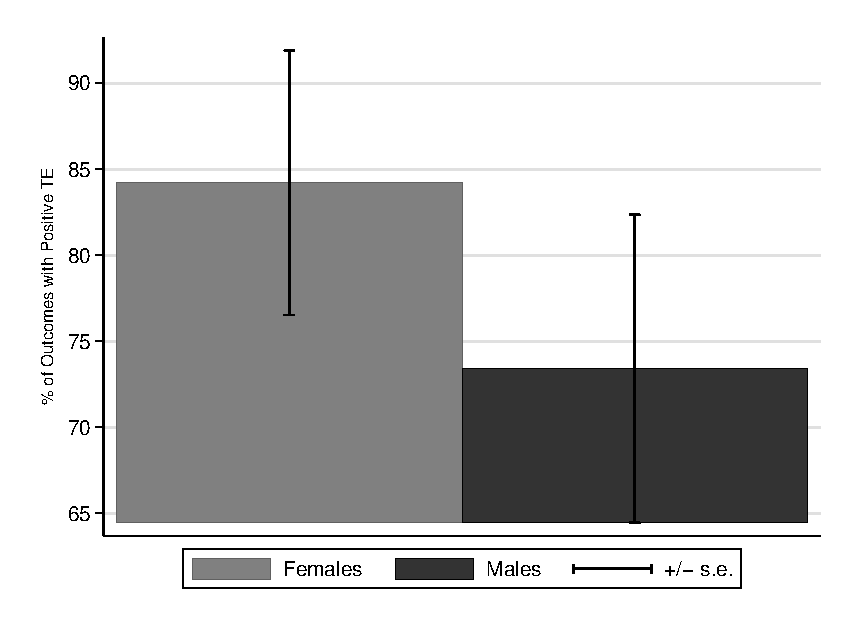
\includegraphics[width=\textwidth]{output/itt_noctrl_all.eps}
\end{subfigure}%
\begin{subfigure}[h]{0.4\textwidth}
	\centering
	\caption{Treatment vs. Next Best, Significant at 10\% Level} \label{fig:ppositive10}
		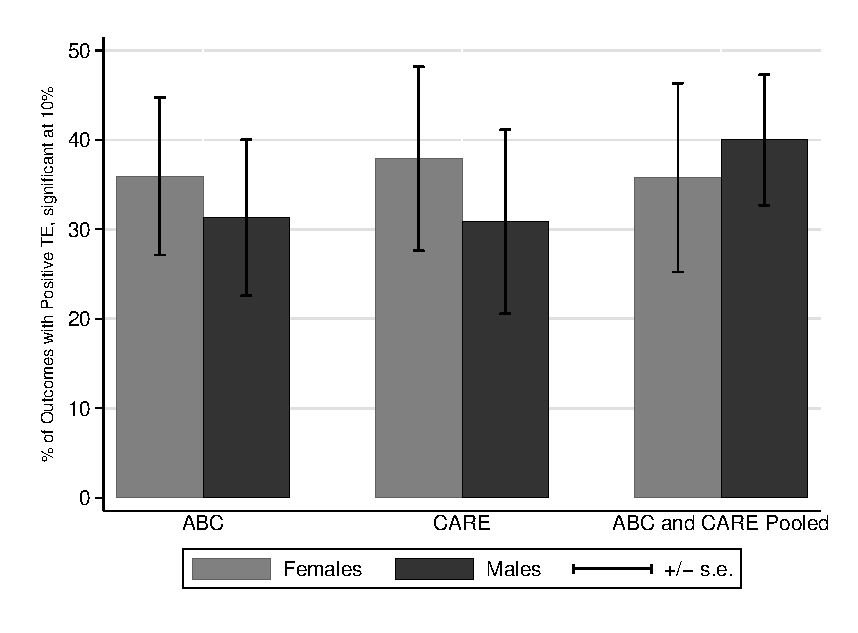
\includegraphics[width=\textwidth]{output/itt_noctrl_all_sig10.eps}
\end{subfigure}
\begin{subfigure}[h]{0.4\textwidth}
		\centering
		\caption{ Treatment vs. Stay at Home} \label{fig:ppositivehome}
		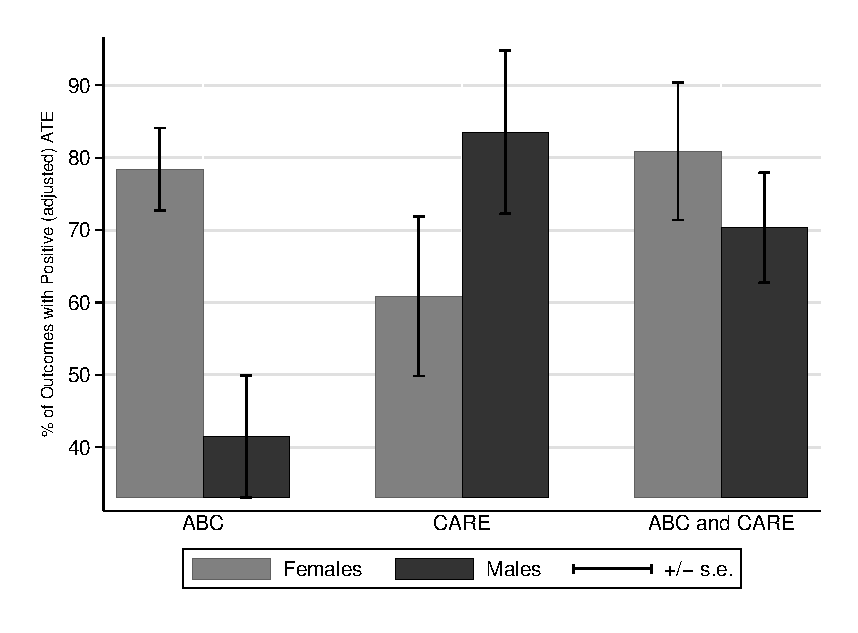
\includegraphics[width=\textwidth]{output/epan_ipw_p0_all.eps}
\end{subfigure}%
\begin{subfigure}[h]{0.4\textwidth}
	\centering
	\caption{Treatment vs. Alternative Preschool} \label{fig:ppositivealternative}
		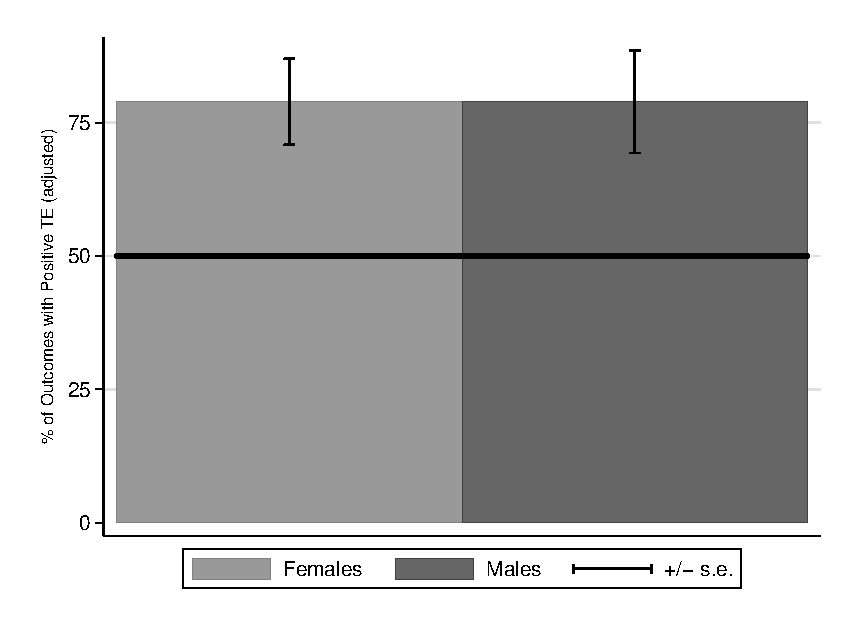
\includegraphics[width=\textwidth]{output/epan_ipw_p1_all.eps}
\end{subfigure}
\scriptsize \justify
Note: Panel (a) percentage of outcomes displaying a positive treatment effect, comparing treatment to next best. Panel (b) percentage of outcomes displaying a positive and statistically significant treatment effect (10\% significance level). Panel (c) displays the percentage of outcomes with a positive treatment effect, comparing treatment to staying at home. Panel (d) displays the percentage of outcomes with a positive treatment effect, comparing treatment to alternative childcare arrangements. Standard errors are based on the empirical bootstrap distribution. For Panel (b) we perform a ``double bootstrap'' procedure to first determine significant treatment effects at $10\%$ level and then calculate the standard error of the count.\\
\end{sidewaysfigure}

Finally, we present the estimates of the combining functions by outcome category. Figure~\ref{fig:cats-positive-significant} shows the estimated proportions that are statistically significantly positive at the 10\% level. Consistent with the treatment effects above, control-group females tend to do better in alternative childcare than at home. This is especially true for parenting measures, IQ, education, and employment. Control-group males, on the other hand, do better at home, with more positive treatment effects compared to low quality childcare.

\begin{figure}[H]
\centering
\caption{Proportion of Positively Impacted Outcomes by Category, ABC/CARE Males and Females}\label{fig:cats-positive-significant}
\begin{subfigure}[h]{0.7\textwidth}
	\centering
	\caption{Treatment vs. Stay at Home, Significant at 10\% Level}
		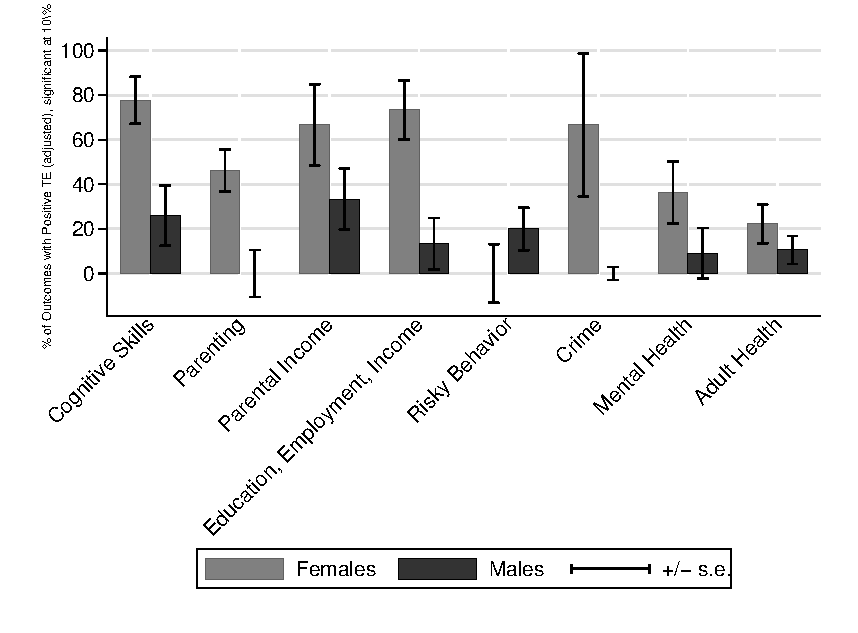
\includegraphics[width=\textwidth]{output/epan_ipw_p0_cats1_sig10.eps}
\end{subfigure}

\begin{subfigure}[h]{0.7\textwidth}
	\centering
	\caption{Treatment vs. Alternative Preschool, Significant at 10\% Level}
		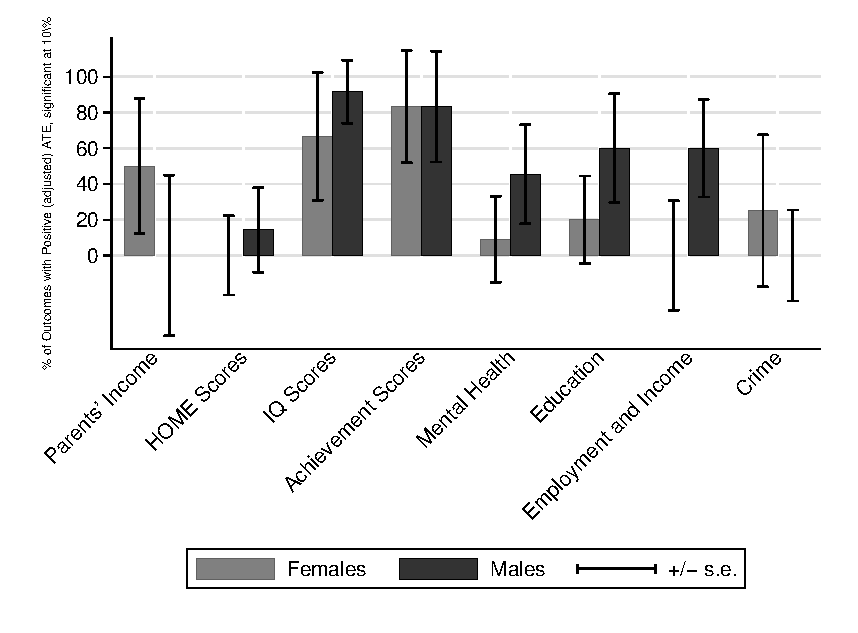
\includegraphics[width=\textwidth]{output/epan_ipw_p1_cats1_sig10.eps}
\end{subfigure}
\scriptsize \justify
Note: Panel (a) percentage of outcomes displaying a positive treatment effect, comparing treatment to next best. Panel (b) percentage of outcomes displaying a positive and statistically significant treatment effect (10\% significance level). Panel (c) displays the percentage of outcomes with a positive treatment effect, comparing treatment to staying at home. Panel (d) displays the percentage of outcomes with a positive treatment effect, comparing treatment to alternative childcare arrangements. Standard errors are based on the empirical bootstrap distribution. For Panel (b) we perform a ``double bootstrap'' procedure to first determine significant treatment effects at $10\%$ level and then calculate the standard error of the count.\\
\end{figure}

